\chapter{Ensayos y Validaciones}
La prueba inicia cargando los datos base, como el nombre de la Organización, las áreas que responsables de los eventos que emitirán los documentos.
Partiendo de un smart contract desplegado como se mostrá en otras secciones, el administrador o propietario de la organización concuerda con la dirección encargada 
de publicar el contrato inteligente, pero este puede ser cambiado por otro.
\section{Ajustando el Sistema}

Se cambia el nombre de la organización a “ Universidad Nacional de Misiones Facultad de Ciencias Económicas ”, esto sirve para identificar el nombre de la organización, se 
crean estados nuevos como “ en espera ”, “ on hold ” \ref{img:cambio_org}.
Se crean las Áreas de la Organización, es este caso “ Secretaría de Extensión ” , con el propietario del área con dirección  “ 0x255A43ac4ed05F41396 07B33523a591ACE5a4031”
y el estado “ actived ”, conforme a la figura  \ref{img:nuva_area}.
\begin{figure}[H]
  \centering
  {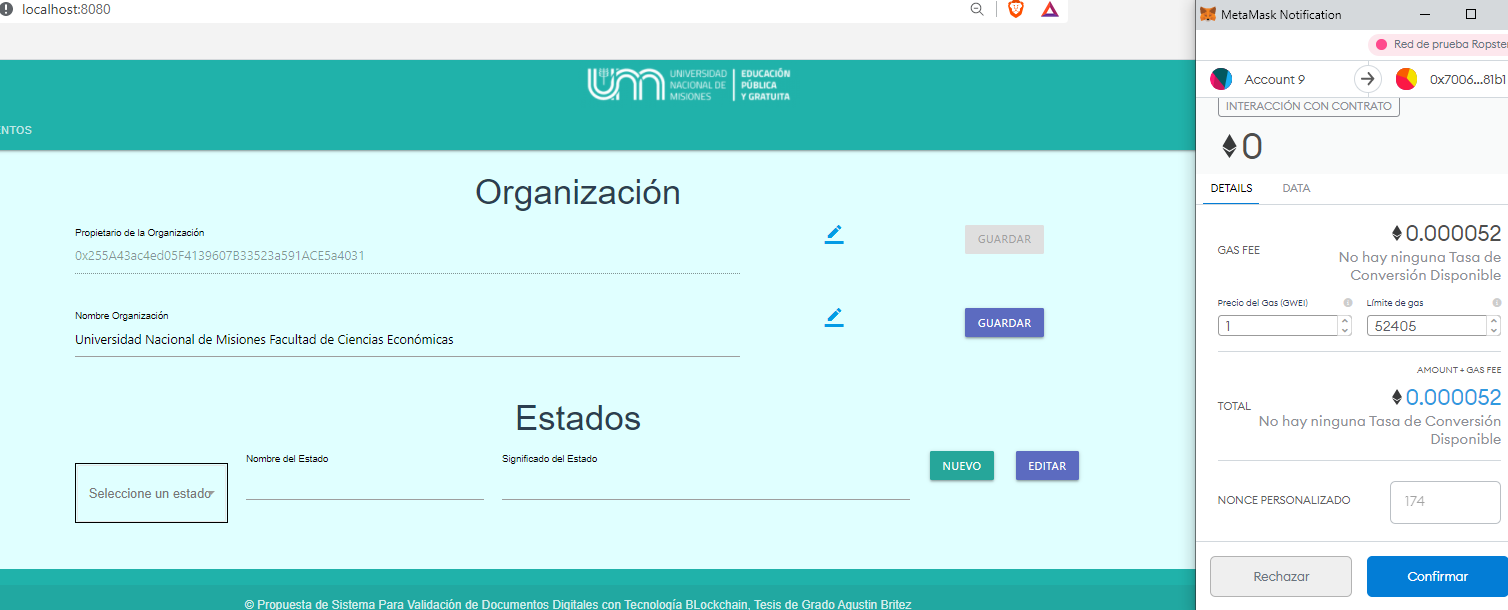
\includegraphics[scale=0.4]{cambio_organizacion.png}}
  \caption{Cambio de nombre de la organización,  Fuente: captura de pantalla. }
  \label{img:cambio_org}
\end{figure}

\begin{figure}[H]
  \centering
  {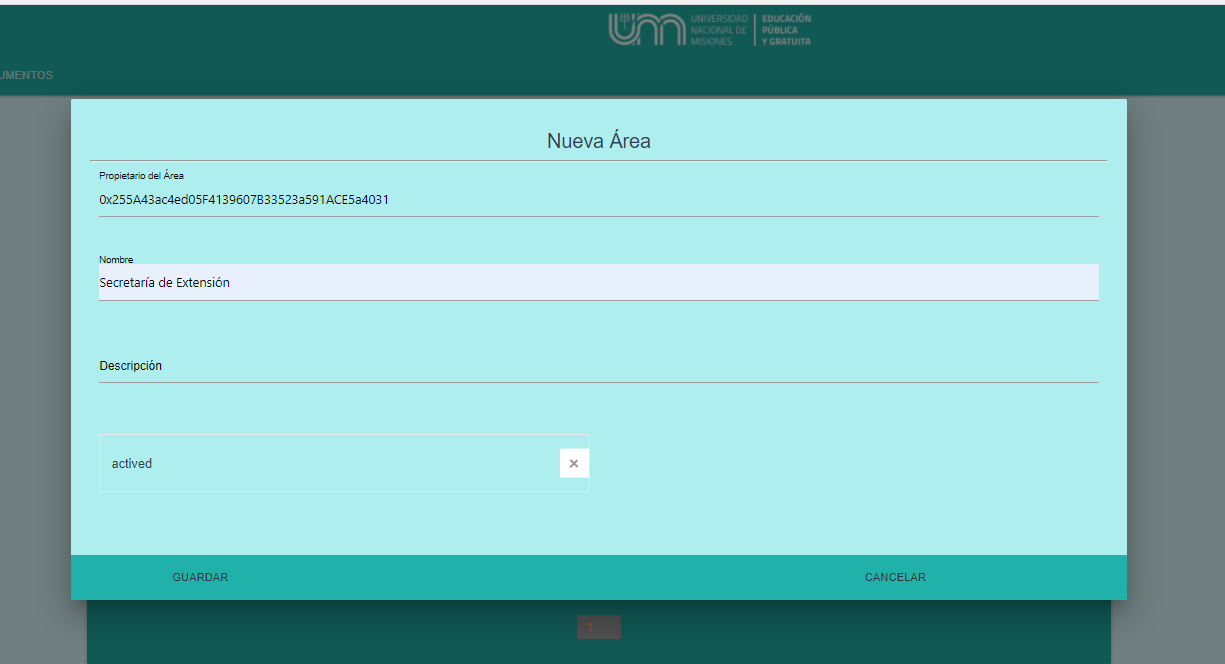
\includegraphics[scale=0.4]{nueva_area.png}}
  \caption{Creación de nueva área en el sistema,  Fuente: captura de pantalla. }
  \label{img:nuva_area}
\end{figure}
Se requiere una actividad  el cual genera los documentos, por ende se crea uno con el nombre de “ Curso de Economía Actual ” , que se relaciona al área recién mencionada que es 
“ Secretaría de Extensión ” con una fecha de inicio del evento el “ 18/05/2021 08:00hs” y fecha de finalización “ 20/05/2021 08:00hs ”.
\begin{figure}[H]
  \centering
  {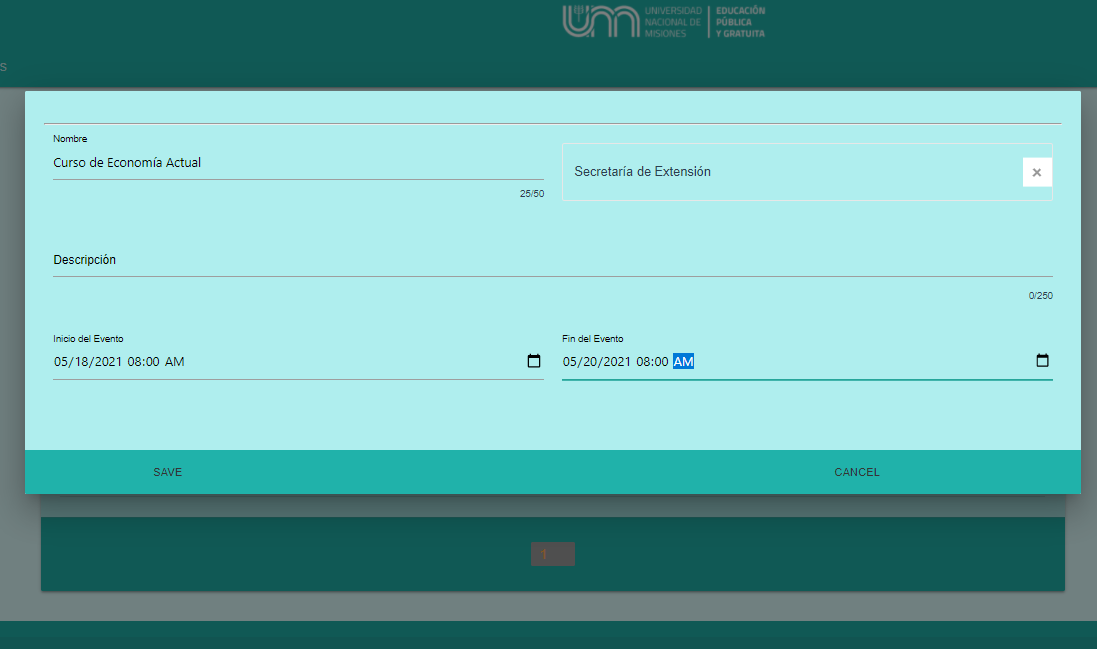
\includegraphics[scale=0.4]{nuevo_evento.png}}
  \caption{Creación de nueva área en el sistema,  Fuente: captura de pantalla. }
  \label{img:nuevo_evento}
\end{figure}




\subsection{Validación de Documento}

Se ensayará en un flujo habitual de la Secretaría de Extensión de la \glsfirst{fce}, 
siguiendo los circuitos normales de una actividad realizada por esta área. En base a la información recaudada en la entrevistas\cite[]{larraburu_secretariextension_2020},
  comenzando el flujo desde el momento que se crea un documento digital para entregar 
al participante de una actividad.

Los pasos previos antes de  enviar o entregar el documento digital al participante son: 
\begin{enumerate}
  \item Sellar el documento en la Blockchain, en la vista “ encontrar documento ” , con la Metamask tener la cuenta del 
  propietario del área activada.
  \item Seleccionar el Área de “ Secretaría de Extensión ” y el Evento “ Curso de Economía Actual ”, el resto de los input se deja vacío.
  \item Luego se da click al botón “ DOCUMENTOS ” y se selecciona los documentos para  generar el hash y almacenarlo en la Blockchain, en el ejemplo de la figura \ref{img:nuevos_certificados} se muestran 3 certificados seleccionados
  que aun no están verificados porque no se encuentran almacenados, se puede observar que el hash de cada uno es diferente, los certificados subidos 
  se pueden ver en el anexo \ref{as:imagenes_pruebas}.
  \begin{figure}[H]
    \centering
    {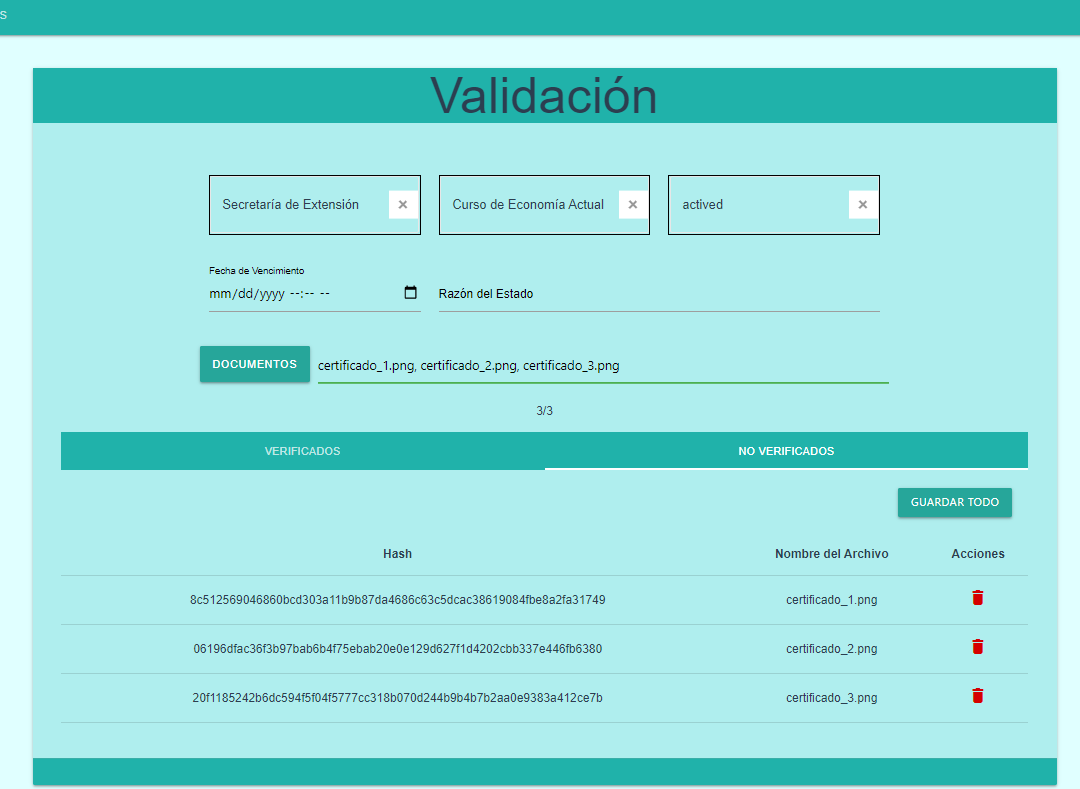
\includegraphics[scale=0.5]{prueba_cargando_certificados.png}}
    \caption{Carga de nuevos documentos,  Fuente: captura de pantalla. }
    \label{img:nuevos_certificados}
  \end{figure}
  \item  El siguiente paso es dar click en el botón “ GUARDAR TODO ”, esto almacena los datos cargados en la Blockchain.
  \item Una vez completada la transacción en la  Blockchain de prueba, los documentos aparecen como verificados (ver Figura \ref{img:prueba_almacenamiento}).
  \begin{figure}[H]
    \centering
    {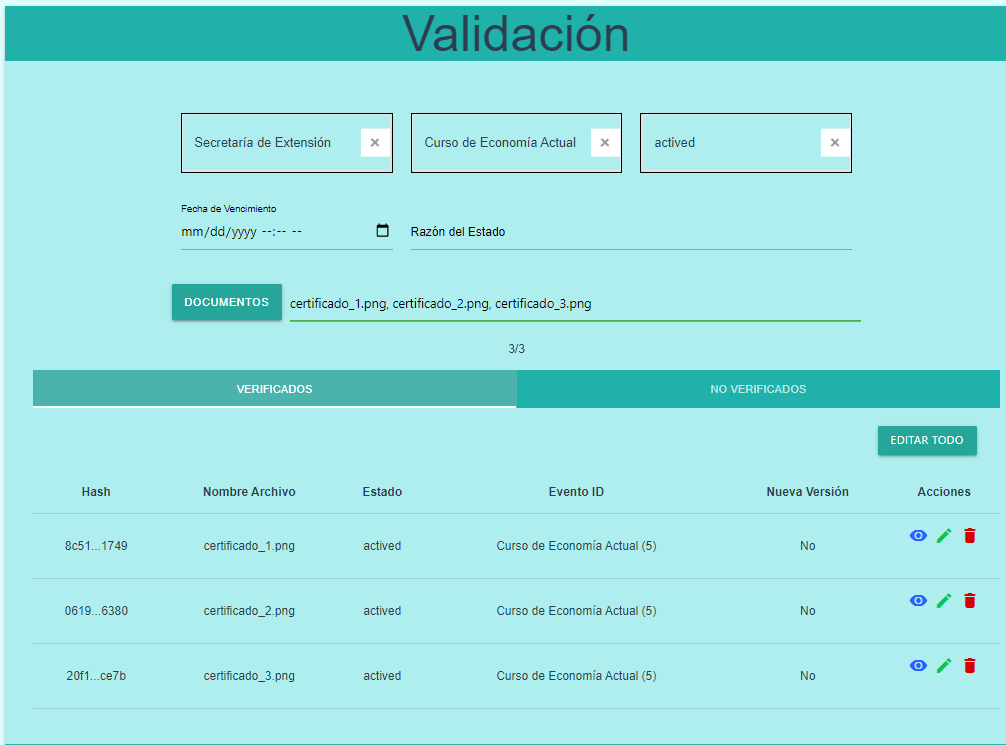
\includegraphics[scale=0.5]{prueba_documento_almacenado.png}}
    \caption{Hash de documentos almacenados y verificados,  Fuente: captura de pantalla. }
    \label{img:prueba_almacenamiento}
  \end{figure}
\end{enumerate}
Finalizado los pasos la organización puede enviar los documentos sellados en la  Blockchain , ya que estos
podrán ser validados posteriormente.

Por otro lado para consultar si el contenido del certificado no ha sido alterado, se 
sube el documento accediendo al apartado “ DOCUMENTOS ”   y si aparece en la sección verificado
es porque si fue almacenado por la organización en este caso la \gls{unam}-\gls{fce}
En la figura \ref{img:sin_metamask} se consultan todos los documentos subidos en los pasos de la prueba , sin tener  una wallet y los datos
son visibles permitiendo libre acceso. 
\begin{figure}[H]
  \centering
  {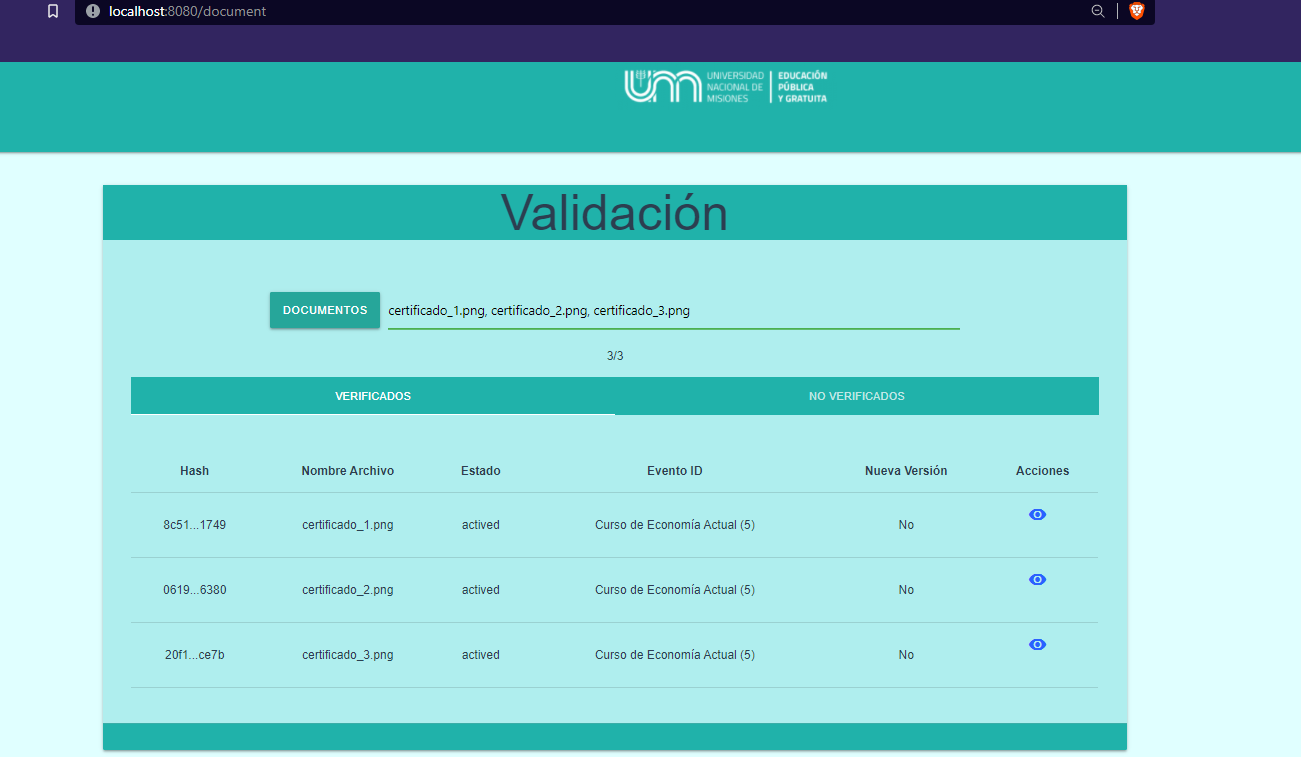
\includegraphics[scale=0.5]{sin_metamask.png}}
  \caption{Validación de documentos,  Fuente: captura de pantalla. }
  \label{img:sin_metamask}
\end{figure}


El flujo cuenta con escasos pasos dando potencial para  verificar los documento sin registrase o aportando algún dato personal.
Cualquier usuario sin Metamask podrá verificar el documento. Por ejemplo un tercero que esta ínteresado en saber si el contenido del certificado
es auténtico y no se ha modificado tendrá la oportunidad de comprobarlo utilizando el sistema.
\subsection{Puesta en Practica}

A continuación se realiza una modificación al certificado\_3 de la Figura \ref{img:certificado_modificado}, el certificado superior es el original y el inferior está modificado, se ha agregado un 
punto final luego de la letra B, este pequeño cambio hace que el resultado de la función hash cambie totalmente,
antes el hash era “ 20f1185242b6dc594f 5f04f5777cc318b070d244b9b4 b7b2aa0e9383a412ce7b ” con la modificación se obtuvo “ d420851fc0593c0ab226 a34b45f6ffaf6279502e8cea c70c339e9ac4b51a3009 ”.
Por ende se puede validar si un documento ha cambiado en lo más mínimo o si corresponde con un documento generado por la organización.

\begin{figure}[H]
  \centering
  {
\includegraphics[scale=0.5]{certificado_modificado.png}}
  \caption{Modificación de certificado\_3,  Fuente: captura de pantalla. }
  \label{img:certificado_modificado}
\end{figure}

Cuando se carga el certificado modificado, el sistema intenta encontrar el hash  en la Blockchain. Al no estar almacenado lo muestra 
como un certificado no verificado.
\begin{figure}[H]
  \centering
  {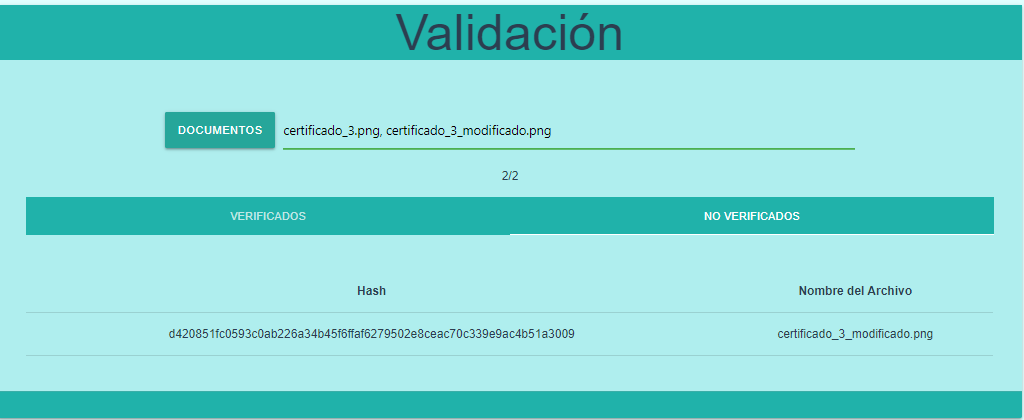
\includegraphics[scale=0.5]{certificado_modificado_novalido.png}}
  \caption{Resultado de la consulta del certificado modificado,  Fuente: captura de pantalla. }
  \label{img:certificado_modificado_consulta}
\end{figure}

Las pruebas demostrada en el flujo fueron con documentos generados, pero a continuación se 
realizan las pruebas con documentos emitidos por la \glsfirst{fce}, (los datos privados de los propietarios 
de los documentos han sido ocultos).

La  prueba se realiza con distintos  documentos PDFs .
\begin{figure}[H]
  \centering
  {
\includegraphics[scale=0.7]{certificado-unam-fondos-buitres.png}}
  \caption{Disertación Fondos Buitres, documento aportado por la Secretaría de Extensión de la \gls{fce} \cite[]{larraburu_secretariextension_2020}}
  \label{img:certificado-unam-fondos-buitres}
\end{figure}

\begin{figure}[H]
  \centering
  {
\includegraphics[scale=0.7]{certificado-unam-liqidacion.png}}
  \caption{Curso de liquidación ingresos brutos y Form. RG 08/2010, documento aportado por la Secretaría de Extensión de la \gls{fce} \cite[]{larraburu_secretariextension_2020}}
  \label{img:certificado-unam-liqidacion}
\end{figure}

\begin{figure}[H]
  \centering
  {
\includegraphics[scale=0.7]{certificado-unam-geogebra.png}}
  \caption{Geogebra una herramienta para la resolución de aplicaciones en administración, economía y
  finanzas: un estudio exhaustivo de las funciones, documento aportado por la Secretaría de Extensión de la \gls{fce} \cite[]{larraburu_secretariextension_2020}}
  \label{img:certificado-unam-geogebra}
\end{figure}

Los tres documentos son cargados en la  Blockchain en sus eventos correspondiente, luego se vuelven a cargar
para validar si han sido almacenados, como se observa en la figura \ref{img:Validacion_documentos_UNAM}

\begin{figure}[H]
  \centering
  {\includegraphics[scale=0.7]{Validación_documentos_UNAM.png}}
  \caption{Prueba de generación de hash a partir de documentos de la \gls{unam}, documento aportado la Secretaría de Extensión de la \gls{fce} \cite[]{larraburu_secretariextension_2020}}
  \label{img:Validacion_documentos_UNAM}
\end{figure}

Con esto se comprueba que el sistema soporta los documentos del ámbito académico investigado.



Para verificar si el sistema soporta diferentes tipos de archivos se realizan diferentes tipos de 
pruebas que serán detalladas en la sección de resultados \ref{s:resultados}.



\section{Resultados}\label{s:resultados}


La prueba de validación de documento se realizó con diferentes tipos de documentos en los que se cambiaron el contenido (agregando nuevos 
caracteres como números, letras o símbolos), cinco de tipo texto, cinco de tipo imagen (.png) y cinco de tipo pdf. En todos se realizaron pequeños 
cambios y los resultados
fueron los mismo el hash cambió con el mínimo datos agregados. 
Los resultados de estas pruebas pueden observarse en la tabla \ref{table:tabla-prueba}, y los contenidos de los archivos se encuentran en el anexo \ref{as:elementos_prueba}.

Las validaciones con  los documentos con extensión .TXT son:

Los archivos de textos y pdfs utilizados en las pruebas contenían la siguiente información.
    \begin{table}[H]
    \centering
    % l = lefht c=centrado r=right
    \begin{tabular}{ |l|c|r| }
    \hline
    Archivo & Contenido Original & Contenido Modificado \\
    \hline
    text1.TXT & Prueba de texto  & Prueba de texto  \\
              &  para certificado & para certificado. \\
    \hline
    text2.TXT & Prueba numero dos  & Prueba numero dos  \\
              &  para texto & para texto.. \\
    \hline
    text3.TXT & Este texto es          & Este texto es  \\
              &  diferente a los demas & diferente a los demás \\
    \hline
    text4.TXT & El estudiante aprobo  & El estudiante aprobó  \\
     & la materia & la materia \\
    \hline
    text5.TXT & Textos con simbolos .  & Textos con símbolos .  \\
     &  / \_ () 1234567890 +=[] & / \_ () 1234567890 +=[1] \\
    \hline
    \end{tabular}
    \caption{Contenido de los textos}
    \label{table:tabla-textos-prueba}
    \end{table}

\begin{table}
  \centering
  % l = lefht c=centrado r=right
 
  \begin{tabular}{ |l|c|c|l| }
    \hline
    nombre del documento & hash documento original & hash documento modificado  & Hay alteración\\
  \hline
  text1.TXT & b57e3546fbafe53bfb8b6eb7& b434a503c6592a7f9df4ce    & SI\\
            & 8f38e77361c5db8fc82435f8& c461d20f60e444fa59fc19e   & SI\\
            & 3ea67143d56449f0        & 042afe3b2be9a072265      & SI\\
  \hline
  text2.TXT & a55fa0b329d07798be5826f & beef2d16c441f6d919982  & SI\\
            & f196aca6badd94226dc9a35 & 0d06116532bafaedf89b2  & SI\\
            & 6f414f6c6356fbee75      & b9dfe6f60a6367ad81bfa6  & SI\\
  \hline
  text3.TXT & d1a7d4f67a558c981eda061 & 3e200092a6fb306610eea  & SI\\
            & 26f3979cbd581d345011e5e & 52ba76dab08f520d5dc7b  & SI\\
            & a81b3e40924505c402      & 57e181ba444b2f67ccaed8  & SI\\
  \hline
  text4.TXT & 6822f8bf26013b72ea0e019 & aacf42b244e6078c93f2c & SI\\
            & 8f80ff5a82f574312456b98 & c6e561a7081a570101475& SI\\
            & 060bab6d71d40e1dcd      & 3d390f987ed8883f7ff7fd & SI\\
  \hline
  text5.TXT & 651d9bfd2f13d17989fd44d & c1f3886ff37a702c3434a & SI\\
            & 9b10eacfea00202dd043419 & 50e8c1d6ce8035f6f3d02 & SI\\
            & 01eb572572da4c188b      & 21b101cccd42a9351b9e55 & SI\\
            \hline
            text1.pdf & 0c4baf3336bfd3d4a7bc47e & 350c84015656f8cccaa93 & SI\\
                      & c84521d6018956d09a74e20 & 1174a8154e38ac56ce025 & SI\\
                      & befe724d919988ca49      & 161440a0d104e2f6c8e8b6 & SI\\
            \hline
            text2.pdf & 3e924183b92015b3540eb12 & 3419acb9640a35d173020 & SI\\
                      & ce7ce0dabf2fce19574f462 & 12d9dacbb7bc399884651 & SI\\
                      & 2bd79dcd907592c930      & 50fb189d92981d5bf91cfc & SI\\
            \hline
            text3.pdf & 093d0bbb1ba9196713d4d71 & 48d94e4936fa1696d7d20	 & SI\\
                      & 024b095cab07ac4efda5b0e & 7cb89189e7b3e1256ae05 & SI\\
                      & 5a1d0b89ec19426db3      & b299399d2dbd372da8d420 & SI\\
            \hline
            text4.pdf & 08c45f59b18d5080ff20efe & 98f9b10cd295e807ff42b & SI\\
                      & 2a7b2510f30ed6f528eb39b & 19a40a3fd32824f8f3b75 & SI\\
                      & 603267254a5fbe71ec      & f9bddb553acad24e6e5b5e & SI\\
            \hline
            text5.pdf & 90a2d6b01745b172655a845 & d31ef2d892f9fb388788 & SI\\
                      & 260b0b67302b6ffa3860554 & 315985dbee28fdad03b90 & SI\\
                      & 6443a9a341278b020e      & c41902472631a8f3449932d & SI\\
  \end{tabular}
  \caption{Resultados de las pruebas}
  \label{table:tabla-prueba}
  \end{table}

\begin{table}
  \centering
  % l = lefht c=centrado r=right
 
  \begin{tabular}{ |l|c|c|l| }
    \hline
    nombre del documento & hash documento original & hash documento modificado  & Hay alteración\\
  \hline
  text1.pdf & 0c4baf3336bfd3d4a7bc47e & 350c84015656f8cccaa93 & SI\\
            & c84521d6018956d09a74e20 & 1174a8154e38ac56ce025 & SI\\
            & befe724d919988ca49      & 161440a0d104e2f6c8e8b6 & SI\\
  \hline
  text2.pdf & 3e924183b92015b3540eb12 & 3419acb9640a35d173020 & SI\\
            & ce7ce0dabf2fce19574f462 & 12d9dacbb7bc399884651 & SI\\
            & 2bd79dcd907592c930      & 50fb189d92981d5bf91cfc & SI\\
  \hline
  text3.pdf & 093d0bbb1ba9196713d4d71 & 48d94e4936fa1696d7d20	 & SI\\
            & 024b095cab07ac4efda5b0e & 7cb89189e7b3e1256ae05 & SI\\
            & 5a1d0b89ec19426db3      & b299399d2dbd372da8d420 & SI\\
  \hline
  text4.pdf & 08c45f59b18d5080ff20efe & 98f9b10cd295e807ff42b & SI\\
            & 2a7b2510f30ed6f528eb39b & 19a40a3fd32824f8f3b75 & SI\\
            & 603267254a5fbe71ec      & f9bddb553acad24e6e5b5e & SI\\
  \hline
  text5.pdf & 90a2d6b01745b172655a845 & d31ef2d892f9fb388788 & SI\\
            & 260b0b67302b6ffa3860554 & 315985dbee28fdad03b90 & SI\\
            & 6443a9a341278b020e      & c41902472631a8f3449932d & SI\\
  \hline
  \end{tabular}
  \caption{Resultados de las pruebas}
  \label{table:tabla-hash-pdf}
  \end{table}
  
  \begin{table}
    \centering
  \begin{tabular}{ |l|c|c|l| }
    \hline
    nombre del documento & hash documento original & hash documento modificado  & Hay alteración\\
  \hline
  imagen1.png & 10a099a6393881be73909 & c6148ecbef63337577da8 & SI\\
            & 47c22161dbe618d1739f3ad & 12bec203f6a92a0aad756 & SI\\
            & 6dc80d8fb3fc918cda11    & 3c246f3a8213404b54cd9c & SI\\
  \hline
  imagen2.png & 814ce95d3aa3e31a6b949 & b95ec390073d820902ee6 & SI\\
            & 6d2aae10b0685878b2a913d & d3ccf48e52c65d01bba32 & SI\\
            & 130696d23ef6a5ef5c08    & 0ef508dee2e5b4918ae485 & SI\\
  \hline
  imagen3.png & f9fc277e29e010b82703b & 155ff7434bfbc94aa116f	 & SI\\
            & dbb72781b102a0e999e2242 & 76462f6206611bf40cab5 & SI\\
            & ba363a3d2e3b9eed9901    & d3b90826ad1b3430194ed8 & SI\\
  \hline
  imagen4.png & faa773cdf9371e52290298 & 6306a96ced0e182c89d46 & SI\\
            & 441bf30f64bf04a75791a271 & a19a660812a0337c39f3d & SI\\
            & 5fbc860c80867d73ce       & c6bc86341f194c7f4216f2 & SI\\
  \hline
  imagen5.png & e8c2cd3fc8e831346a4625b  & a9e6aec03772334e9b7 & SI\\
            & 82c866c7086d8bad82bdc07  & 2744927cff6de59f5969a & SI\\
            & 8a7cddb30eaf753ea9     & f3d519b68d2b75002b8f48c7 & SI\\
  \hline
  \end{tabular}
  \caption{Resultados de las pruebas}
  \label{table:tabla-hash-png}
  \end{table}
